\chapter{A Python Package for SMBO} \label{ch:code}


In exploring this topic, I have built a Python package for performing sequential model-based optimization, simply named \texttt{smbo}. My goal in making it was to construct well-made code that will be immediately useful as a pedagogical tool (indeed, it was used to generate several figures in this thesis, such as those in Section \ref{sec:smbo_ex}), open source and available online, and documented and designed such that further development of the code base is easy. Perhaps some day \texttt{smbo} will evolve into a cutting-edge free optimization package, used to optimize all sorts of blackbox functions all over the globe, maintained by an international team of elite open-source hackers. Presently, the project is more humble. As of submitting this thesis, the package only implements the EGO algorithm, though its modular, hybrid object-oriented/functional construction allows for further SMBO processes to be defined and implemented easily. \texttt{smbo} is available on the Python Package Index, and can be downloaded and installed with a single command on any computer with Python 2.7.9 or later.\footnote{\texttt{sudo pip install smbo}}

As a good portion of the work in this thesis went into software design and engineering (subjects not taught at Reed College), I will here present the code behind the \texttt{smbo} package on the highest level. This discussion will inform the reader's mathematical understanding of SMBO processes, covering design decisions, identifying runtime bottlenecks, and the crucial components upon which the performance of any SMBO implementation rely. This chapter will also serve as an introduction to the official documentation of the \texttt{smbo} package, which is included as an appendix to this thesis.

\section{Design}\label{sec:design}

The three-stage SMBO cycle, illustrated earlier in Figure \ref{fig:smbo_cycle}, presents a clear opportunity for a modular package design. As a reminder to the reader, the SMBO loop has three parts: an objective function (i), a modelling method (ii), and a method for additional sample point selection (iii). I will present \texttt{smbo} as it relates to these three steps.

\subsection{\texttt{smb$\_$optimizer}}

The technical goal of the \texttt{smbo} package is to provide a class, called \texttt{smb$\_$optimizer}, which generically handles and passes arguments between each component of the SMBO loop to facilitate iteration of the SMBO process. Since this thesis is largely concerned with the case where (iii) is defined by expected improvement maximization (Section \ref{sec:max_imp}), this stage of the process is implemented by a fixed class method of \texttt{smb$\_$optimizer}, called \texttt{sample}. The other two steps of the loop are implemented as functional properties of each \texttt{smb$\_$optimizer} instance, passed as initialization arguments. This information is illustrated on the familiar SMBO loop in Figure \ref{fig:smbo_loop_II}. Figure \ref{fig:smb_opt_doc} is a summary of the official documentation for the \texttt{smb$\_$optimizer} class, listing all of the high-level methods used in iterating the SMBO loop.

\begin{figure}[h]
	\centering
	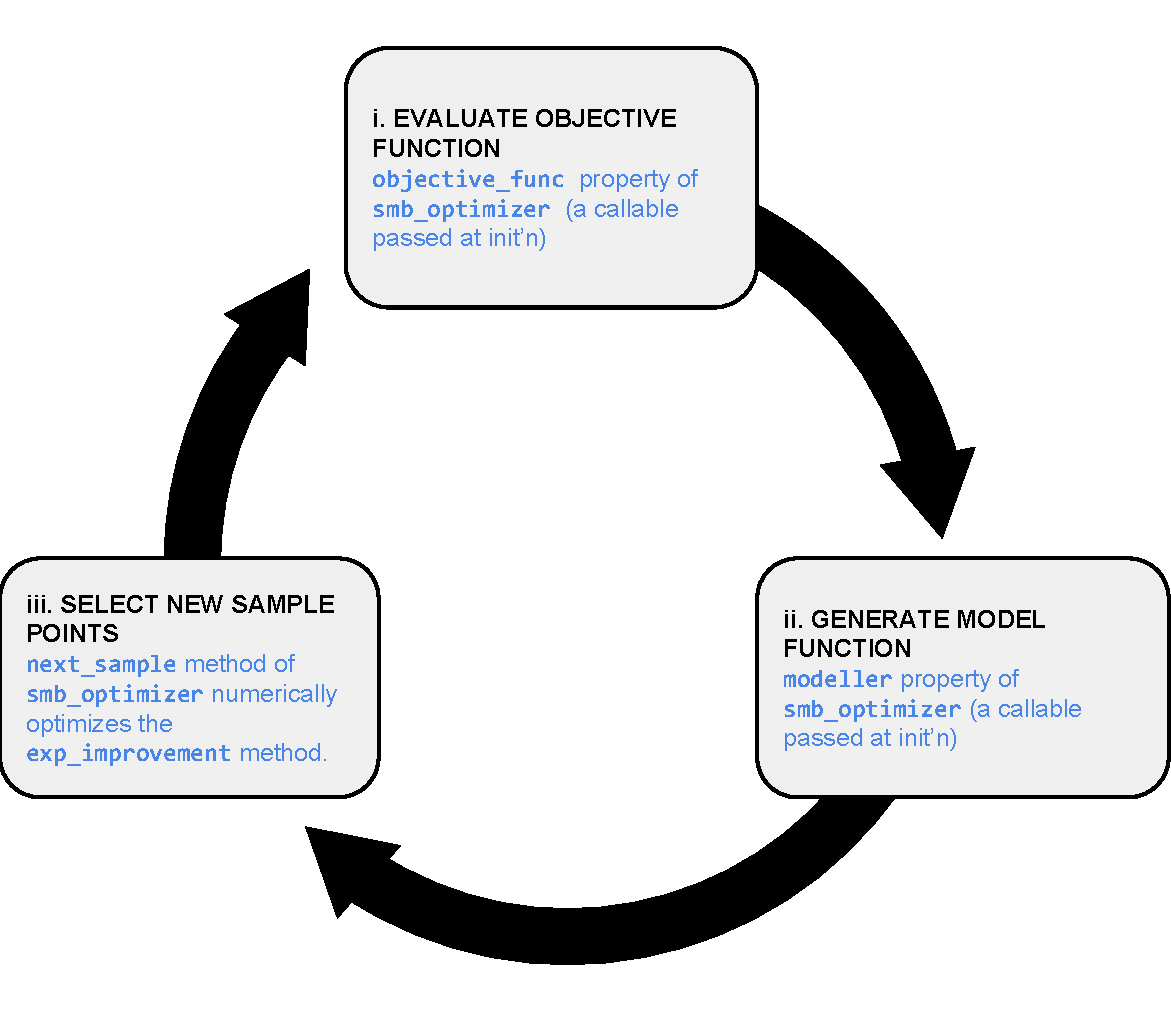
\includegraphics[width=0.75\textwidth]{smbo_loop_II}
	\caption{An instantiation of an SMBO process consists of a single \texttt{smb$\_$optimizer} object. Here the SMBO loop is labeled with the type of its implementation in the \texttt{smb$\_$optimizer} class.}
	\label{fig:smbo_loop_II}

\end{figure}


% The smb_optimizer documentation
\begin{minipage}{\textwidth}
\begin{framed}
\begin{fulllineitems}
\phantomsection\label{index:smbo.smb_optimizer.smb_optimizer}\pysiglinewithargsret{\strong{class }\code{smbo.smb\_optimizer.}\bfcode{smb\_optimizer}}{\emph{domain}, \emph{objective\_func}, \emph{modeller}, \emph{init\_sampler=None}}{}
An object that, given an input domain, objective function, and modelling strategy, implements sequential model-based optimization to search for a global minimum of the objective function.
\begin{quote}\begin{description}
\item[{Initialization Arguments}] \leavevmode\begin{itemize}
\item {} 
\textbf{\texttt{domain}} (\emph{list}) -- a list whose \(i^{th}\) element is the \((lower\ bound,\ upper\ bound)\) pair
describing the domain of interest in the \(i^{th}\) input dimension. The length
of this list defines the dimension of input space, denoted \(k\). This smb\_optimizer
then optimizes the \(k\)-rectangle defined by the domain arg.

\item {} 
\textbf{\texttt{objective\_func}} (\emph{function}) -- a function (or any object with a suitable \_\_apply\_\_ method)
that maps \(k\)-vectors to floats. The goal of an smb\_optimizer is to minimize this
function over the domain defined above.

\item {} 
\textbf{\texttt{modeller}} (\emph{function}) -- a function (or any object with a suitable \_\_apply\_\_ method) that maps a
tuple \((X,Y)\), which describes the input and known output values for a list of sample points to a tuple of functions
\((\hat{y},\ \hat{\sigma}^2)\).
\(\hat{y}\) represents the model's best estimate of \code{objective\_func(X)}, and \(\hat{\sigma}^2\)
is the estimated error of that prediction.

\item {} 
\textbf{\texttt{init\_sampler}} (\emph{function}) -- a function which will select initial sample points, informing the zero-generation model.
If left unspecified, is by default set to a \(2k+2\)-sample latin hypercube over the domain,
created with \code{smbo.latin\_hypercube}.

\end{itemize}


\item[{Attributes---Set at Initialization}] \leavevmode\begin{itemize}

\item{}
\textbf{\texttt{X}} (\emph{list}) -- The list of points where \code{objective\_func} has been evaluated already

\item {} 
\textbf{\texttt{Y}} (\emph{list}) -- The list of associated objective function values.

\item {} 
\textbf{\texttt{pred\_y}} (\emph{function}), \textbf{\texttt{pred\_err}} (\emph{function}) -- The predictor and predicted error surfaces; the output of \code{modeller(X,Y)}.

\item {} 
\textbf{\texttt{f\_min}} (\emph{dict:}\texttt{\{x:\_,y:\_\}}) -- The sample point that is the current known minimum.


\end{itemize}


\end{description}\end{quote}

% expected improvement
\index{exp\_improvement() (smbo.smb\_optimizer.smb\_optimizer method)}

\begin{fulllineitems}
\phantomsection\label{index:smbo.smb_optimizer.smb_optimizer.exp_improvement}\pysiglinewithargsret{\bfcode{exp\_improvement}}{\emph{x\_new}}{}Calculates the expected improvement at \code{x\_new}, by estimating from \code{pred\_y} and \code{pred\_err} the probability that an evaluation of \code{objective\_func} at \code{x\_new} would find a value lower than \code{f\_min}.


\end{fulllineitems}


% sample
\begin{fulllineitems}
\phantomsection\label{index:smbo.smb_optimizer.smb_optimizer.sample}\pysiglinewithargsret{\bfcode{sample}}{}{}
Chooses the next sample point by maximizing \code{exp\_improvement}.
Evaluates \code{objective\_func} there, updating \code{X} and \code{Y}. Updates \code{pred\_y} and \code{pred\_err} to the output of \code{modeller(X,Y)}.
\end{fulllineitems}


% take_samples
\index{take\_samples() (smbo.smb\_optimizer.smb\_optimizer method)}
\begin{fulllineitems}
\phantomsection\label{index:smbo.smb_optimizer.smb_optimizer.take_samples}\pysiglinewithargsret{\bfcode{take\_samples}}{\emph{stopping\_improvement=0.01}, \emph{max\_iters=100}, \emph{plot\_dims=None}}{}
Completes the SMBO loop until the best expected improvement is below \code{stopping\_improvement}, or \code{max\_iters} times. Optionally, produces plots of the prediction and error surfaces at every iteration.
\end{fulllineitems}






\end{fulllineitems}


\end{framed}

\captionof{figure}{A summary of the documentation of the \texttt{smb$\_$optimizer} class.}

\end{minipage}




The EGO algorithm, our prototypical SMBO process, is defined by a particular choice of modeller in ste (ii) of the loop, i.e., the DACE model. This is accomplished by a both a DACE function \emph{and} a class in the \texttt{smbo.modellers} module\footnote{The purpose of the \texttt{modellers} module of the \texttt{smbo} package is to contain various predictive models such as DACE, to serve as step (ii) in the SMBO loop.} This is the primary component of \texttt{smbo} meriting the description ``functional/object-oriented hybrid'' mentioned in the introduction to this chapter.

The class \texttt{dace$\_$model} has various methods to implement the calculations defined and derived in Chapter \ref{ch:ego}, including the formulation of $\hat{f}$ and $\err$. The \texttt{dace\_function} function maps the objective data $(\X,\Y)$ (stored here as properties of the $\texttt{smb\_optimizer}$ instance, \texttt{self.X} and \texttt{self.Y}\footnote{Note that in Python, \texttt{self} denotes the class instance at hand, like \texttt{this} in e.g. Java}) to the model functions $(\hat{f},\err)$, which are returned to the $\texttt{smb\_optimizer}$ and stored as \texttt{self.pred\_y} and \texttt{self.pred\_err}. This and more is illustrated in Figure \ref{fig:dace_doc}, a summary of the documentation for \texttt{dace\_function} and \texttt{dace\_model}. Note that the characteristic parameters $\{p_i\},\{\theta_i\}$ are stored as vectors by the \texttt{dace\_class}, in properties \texttt{self.P} and \texttt{self.Q}, respectively.



% The dace documentation
\begin{minipage}{\textwidth}
\begin{framed}
\begin{fulllineitems}
\phantomsection\label{index:smbo.models.dace}\pysiglinewithargsret{\strong{class }\code{smbo.models.}\bfcode{dace}}{\emph{X}, \emph{Y}}{}
A class that implements the DACE model to produce predictor and error surfaces from sample points
\begin{quote}\begin{description}
\item[{Parameters}] \leavevmode\begin{itemize}
\item {} 
\textbf{\texttt{X}} (\emph{list}) -- a list of input vectors

\item {} 
\textbf{\texttt{Y}} (\emph{list}) -- a list of observed objective values

\end{itemize}

\item[{Returns}] \leavevmode
(pred\_y,pred\_err): two functions, each k-to-1, where k is the dimension of the input space, representing the DACE predictor and predicted error at any point in input space.

\item[{Return type}] \leavevmode
tuple

\end{description}\end{quote}
\index{conc\_likelihood() (smbo.models.dace method)}

\begin{fulllineitems}
\phantomsection\label{index:smbo.models.dace.conc_likelihood}\pysiglinewithargsret{\bfcode{conc\_likelihood}}{\emph{new\_P=None}, \emph{new\_Q=None}}{}~\begin{quote}\begin{description}
\item[{Parameters}] \leavevmode\begin{itemize}
\item {} 
\textbf{\texttt{new\_P}} (\emph{list}) -- an \(n\)-vector resetting the \(p\) parameter of the DACE model

\item {} 
\textbf{\texttt{new\_Q}} (\emph{list}) -- an \(n\)-vector resetting the \(q\) or :math:{}`        heta{}` parameter of the DACE model

\end{itemize}

\end{description}\end{quote}

Returns the statistical likelihood of the current DACE parameters \code{P' and :code:{}`Q', given the data :code:{}`X} and \code{Y}.

\end{fulllineitems}
\end{fulllineitems}

\end{framed}

\captionof{figure}{A summary of the documentation of the \code{dace} model class. } \label{fig:dace_doc}

\end{minipage}

An \code{smb\_optimizer} class instance takes \code{dace\_function} (Fig \ref{fig:fig:dace_doc}) as its \code{modeller} argument. Even though the \code{smb\_optimizer} is only aware of this function, each function call initializes a \code{dace} object, which stays alive behind the scenes as long as its \code{predict} and/or \code{pred\_err} methods are being actively called, which is often, as these form the \code{pred\_y} and \code{pred\_err} attributes of the \code{smb\_optimizer}.


There were two factors that influenced the decision to implement the DACE model in this function-wrapped-class kind of way. First, there is the standard conceptual appeal of functional programming---here, we can appreciate the mathematical purity of a code module that behaves exactly as the generic modelling function $M$ described above, mapping sample points to predictive models. This also makes clear the modular distinction between the central \texttt{smb$\_$optimizer} instance and its \texttt{modeller} attribute---as far as an \texttt{smb$\_$optimizer} instance is concerned, the modeller is a black box function which produces models from sample points. On the other hand, the functional paradigm makes it awkward to allow an \texttt{smbo} package user to experiment with the specifics of a particular modelling function, e.g. to see the results of modifying traditionally internal DACE parameters, such as the characteristic parameter vectors \texttt{self.P} and \texttt{self.Q}, which define the shape of the response surface, as described in Section \ref{sec:dace}. For example, the statefulness of the \texttt{dace} class allowed my advisor and I to build our intuition regarding the DACE model, by modifying the normally-behind-the-scenes \texttt{dace} class instance underlying a particular \texttt{smb$\_$optimizer}, and seeing the effects of that change on the plots produced by the \texttt{smb$\_$optimizer}.






\section{Optimization Subroutines}\label{sec:sub_opt}
Each SMBO loop of the EGO algorithm involves two global optimization steps as subroutines. First, the actual fitting of a DACE model to the data is done by selecting the parameters $\mathbf{P}$ and $\mathbf{Q}$ to maximize the likelihood of the data.\footnote{As described in Section \ref{sec:max_lik}, and implemented in \texttt{smbo} with the class method \texttt{smbo.models.dace\_class.exp\_improvement}.} Once a model is fit, the next sample point is selected with the SMBO-standard method of maximizing the expected improvement function \footnote{As described in Section \ref{sec:max_imp} and implemented by the class method \texttt{smbo.smb\_optimizer.exp\_improvement}.} It is somewhat striking that in the process of globally optimizing the objective function, these two functions, both defined in terms of the objective data, are globally optimized many times as subroutines. ``How could we possibly optimize efficiently," a naive person might ask, ``if we are required to perform thousands of other optimizations to do so?'' The answer is rather straightforward: it is easy for us to evaluate the likelihood and expected improvement functions many times, so there is no reason not to use standard somewhat-brute-force optimization methods, such as those widely available in open-source optimization libraries. In comparison, the blackbox function we are dealing with could, for example, be an industrial chemical-experiment-performing robot, or the results of a drug trial. It is important to note this relationship: we generate models of the objective function $f$ which are much less expensive than $f$, computationally speaking. We then evaluate these less expensive functions many, many times to make the most of each query of $f$. It might not be surprising, then, that besides the evaluation of the objective function, these optimization steps are the largest computational bottleneck when implementing SMBO.


These two optimizations performed in EGO can take advantage of known mathematical properties of the functions at hand; they do not share the black box assumption of the larger optimization task. The methods of \cite{jones_efficient_1998} in fact don't even optimize the expected improvement function explicitly, but a mathematically simpler function that underestimates improvement and is easier to optimize (see Section 4.1 of \cite{jones_efficient_1998}). It is worth noting that this craftiness is intended to find a good solution more quickly, not necessarily a better solution, to the expected improvement optimization problem. 

For the sake of modularity, and to take advantage of a preexisting high-quality optimizer, I instead solved these optimization problems with the popular and trusted SciPy library for Python \cite{scipy}. A major reason to use SciPy is pragmatic: it can be trusted to find good solutions quickly, both by the user of the \texttt{smb\_optimizer} class and and the prospective user or contributor to the \texttt{smbo} package. As my ambitious goal is for \texttt{smbo} to eventually be an active open-source library, there is also some subjective advantage to affiliating with the most popular optimization library in the Python open-source community; to use the SciPy brand. Most importantly though, this construction is modular in a way that the perhaps craftier method of \citep{jones_efficient_1998} is not; the \texttt{smb\_optimizer} class chooses the next sample points in a way that is agnostic to the mathematics underlying the modeller, and simply dependent on the model surface and its expected error, $(\hat{f},\err)$. 

It is important that these optimization subroutines run well: generic global optimization, such as of the parameter likelihood and expected improvement functions here, is a notoriously hard problem to solve accurately and efficiently. A slow optimizer subroutine obviously increases the time it takes for a single SMBO loop to be computed, but more importantly, a subroutine that returns significantly sub-optimal solutions to the likelihood and expected improvement problems produces bad predictive models. An example of this is illustrated by example in Fig. \ref{fig:opt_compare}, which shows two DACE models fit to the same data, in all respects identical except for the specific choice of SciPy optimizer used to maximize the likelihood of the characteristic DACE parameters. On the left, a fairly poor fit chosen by \texttt{scipy.optimize.minimize} using \texttt{method:'L-BFGS-B'}\footnote{} and otherwise default parameters. On the right, a much better fit chosen by \texttt{scipy.optimize.basinhopping} with \texttt{method:'COBYLA'}. Note that the right prediction model is not only more accurate than the left, in that $\hat{f}$ is closer to $f$, but the variance of its prediction is smaller almost everywhere. The fit of the model produced by \texttt{basinhopping}, which is designed expressly to not be fooled by local optima, is both more accurate and more confident than that made by \texttt{L-BFGS-B}, which would often converge to poor local optima. This is not meant as a robust comparison of these two components of \texttt{scipy.optimize}, but as a demonstration that the choice of optimizer subroutine has a large effect on the performance of \texttt{smbo}.
\begin{figure}
        \centering
        \begin{subfigure}[t]{0.5\textwidth}
                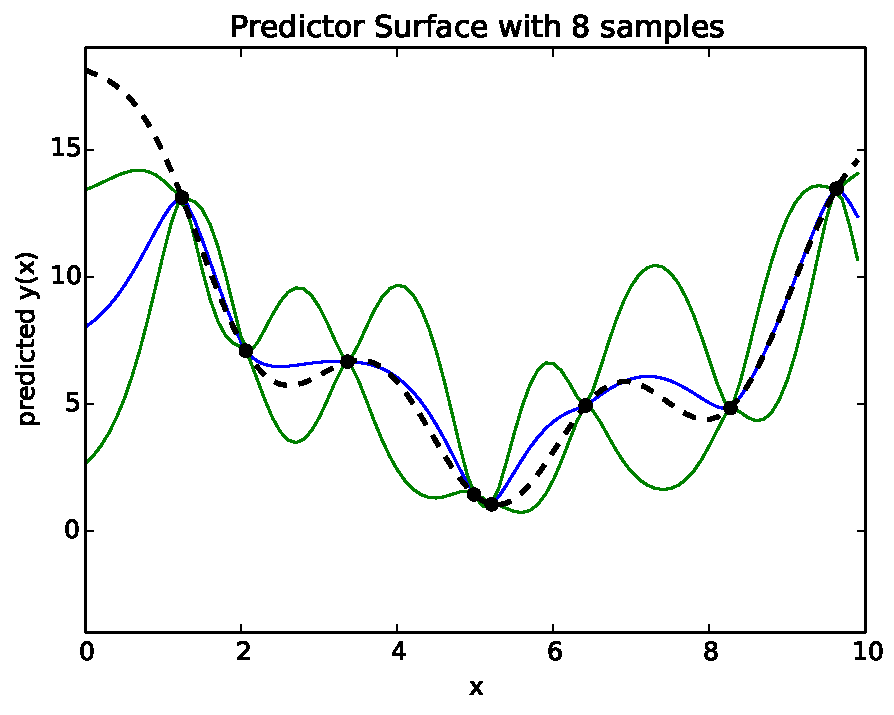
\includegraphics[width=\textwidth]{images/likelihood_opt_ex/bad}
                \caption{L-BFGS-B\cite{}, as implemented by \texttt{scipy.optimize.minimize}. }
        \end{subfigure}%
        ~ %add desired spacing between images, e. g. ~, \quad, \qquad, \hfill etc.
          %(or a blank line to force the subfigure onto a new line)
        \begin{subfigure}[t]{0.5\textwidth}
                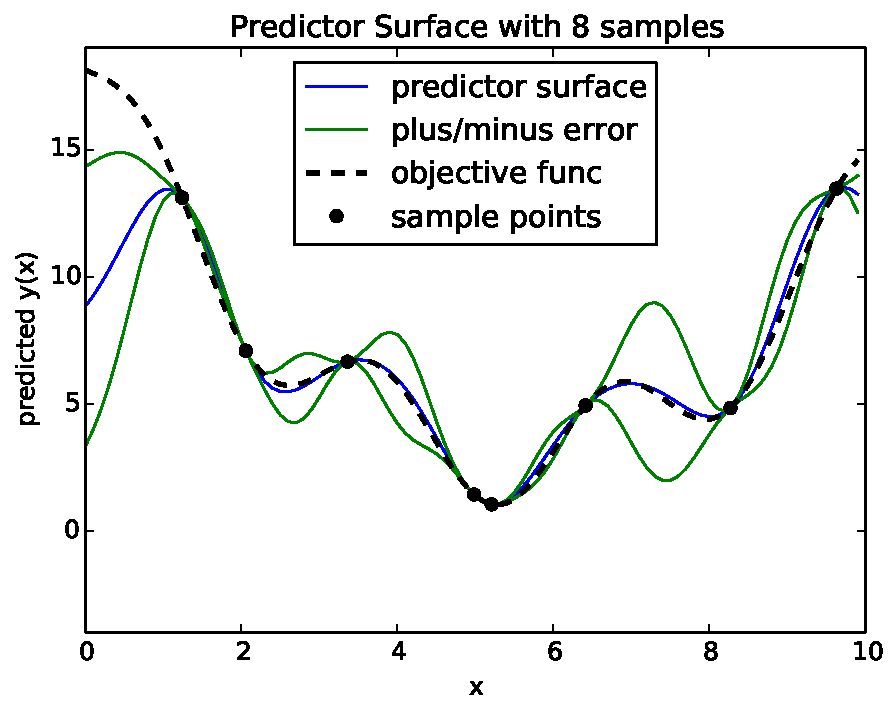
\includegraphics[width=\textwidth]{images/likelihood_opt_ex/good}
                \caption{basinhopping\cite{} global optimization algorithm using COBYLA\cite{} locally, as implemented by \texttt{scipy.optimize.basinhopping}.}
        \end{subfigure}
        \caption{Two DACE predictor models fit to identical sample points, differings only in their method of numeric maximization (labelled) of the parameter likelihood function (Eq. \ref{eq:conc_likelihood}). }\label{fig:opt_compare}
\end{figure}

The optimality of SMBO results depends indirectly, but crucially, on the optimality of the results of these sub-optimizers. The cyclical process works because of each successive model's predictive power in finding the global optimum. The loop is run until, by considering the expected improvement surface, our confidence in having found the global optimum passes a certain threshold. From this we can see that bad predictive models make for an inefficient SMBO loop, because expected improvement is monotonically fixed to predicted error, i.e., more model error means more expected improvement. Poor sub-optimizers make for bad models, which have poor predictive power, which means the SMBO loop will be iterated more times before halting, meaning more calls of the objective function. So, a bad optimizer subroutine will require the objective function to be evaluated more times to get a satisfactory solution to the overall optimization problem. As the premise of this thesis involves a too-expensive blackbox function, this is, of course, bad.

%
%\subsection{Basic Runtime Analysis} \label{sec:runtime}

%Because the premise of this thesis is of an inconveniently-expensive blackbox function, the relevant runtime parameter in this analysis will be the number of objective function evaluations $n$. For convenience, I'll assume that each cycle of the SMBO loop selects only one new sample point, so $n$ is equal to the number of overall SMBO loop iterations.



